%UNIT 10: SPRING MASS SYSTEM AND LINEAR SYSTEMS
%%%%%%%%%%%%%%%%%%%%%%%%%%%
%%%% Put the following at the top of each .tex file  %
\pagestyle{fancy}
\renewcommand{\theUnit}{10}
\ifthenelse{\isundefined{\UnitPageNumbers}}{}{\setcounter{page}{1}}
\rhead{Unit \theUnit: Spring Mass System and Linear Systems}
\lhead{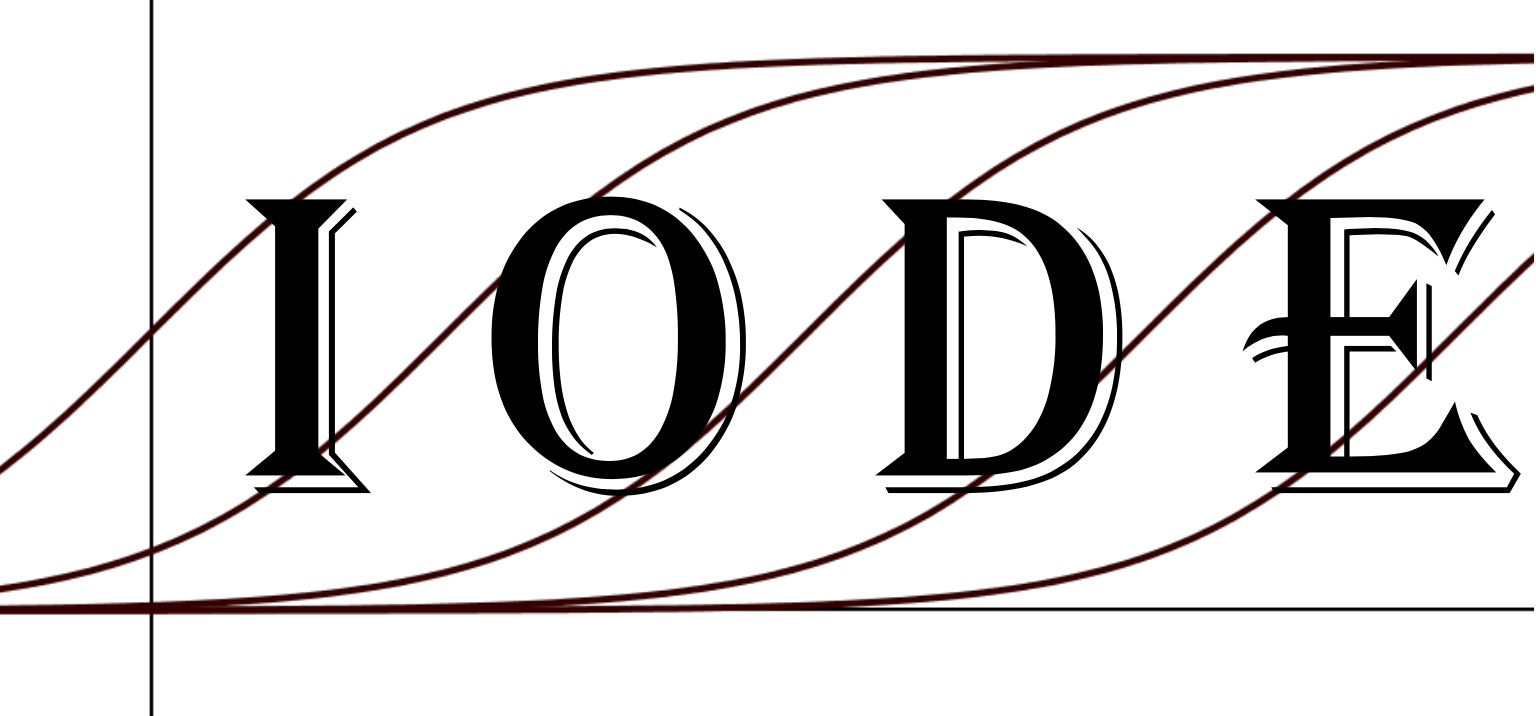
\includegraphics[width=1.25cm]{IODE-logo.png}}
\rfoot{\mypage}
\lfoot{}
\cfoot{}
\fancypagestyle{firstfooter}{\footskip = 50pt}
\renewcommand{\footrulewidth}{.4pt}
%%%%%%%%%%%%%%%%%%%%%%%%%%%
\vspace*{-20pt} \thispagestyle{firstfooter}
\pagebegin{Spring-Mass Motion Investigation}

In this problem we use Newton's Law of motion ($\sum F=ma$ ) to develop a system of rate of change equations in order to be able to describe, explain, and predict the motion of a mass attached to a spring. 

\begin{center}
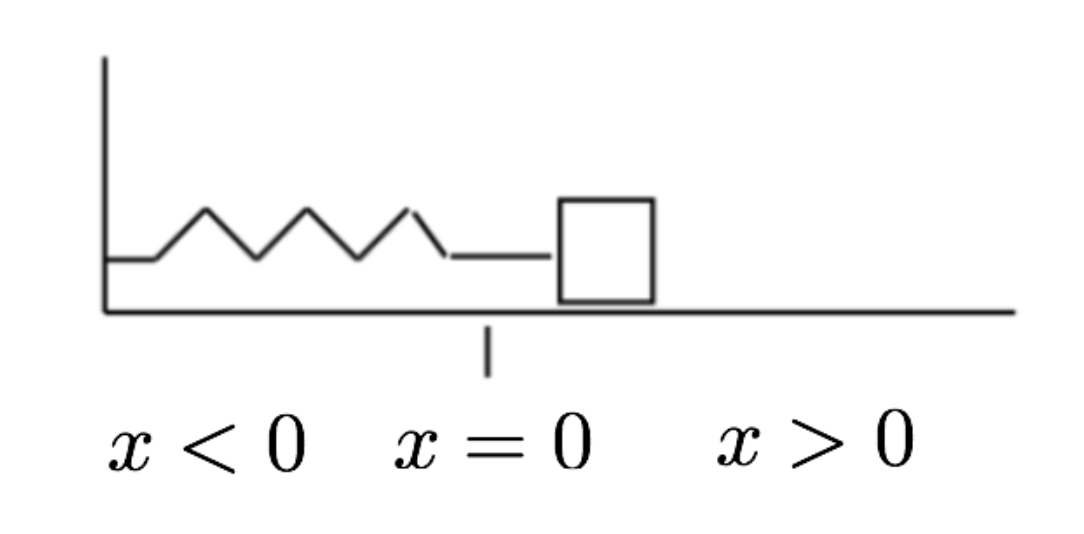
\includegraphics[width=2in]{10/10SpringMass.png}
\end{center}

\begin{enumerate}

\item	Depending on the values for parameters like the stiffness of the spring $k$, the weight of the object attached to the spring $m$, and the amount of friction, different behaviors may be possible. Imagine for a set spring and mass you vary the amount of friction on the surface. What do you imagine the various position versus velocity graphs would look like? Provide rough sketches.\label{10problem1}

\begin{center}
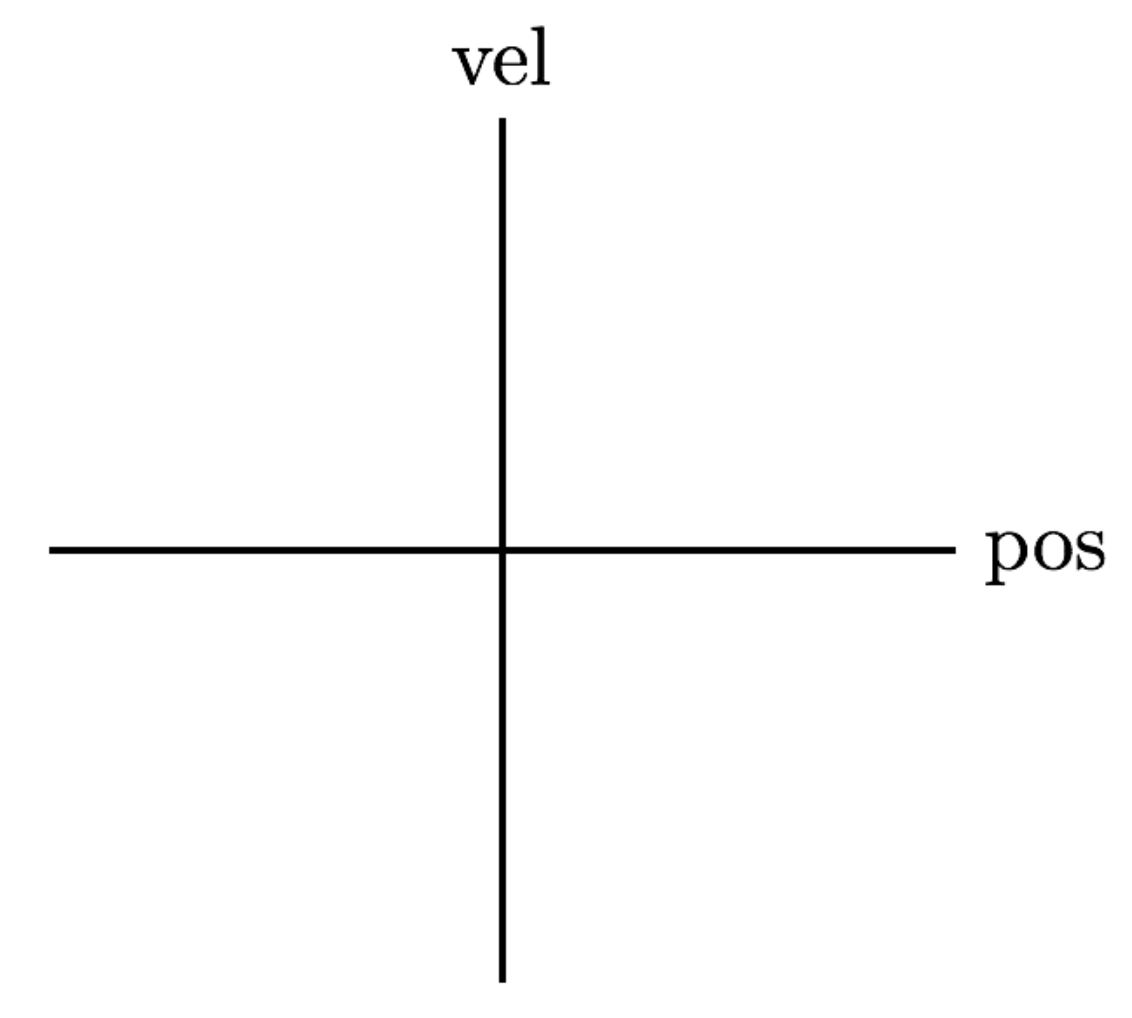
\includegraphics[width=1.75in]{10/10VelPos.png} \hspace{.25in} 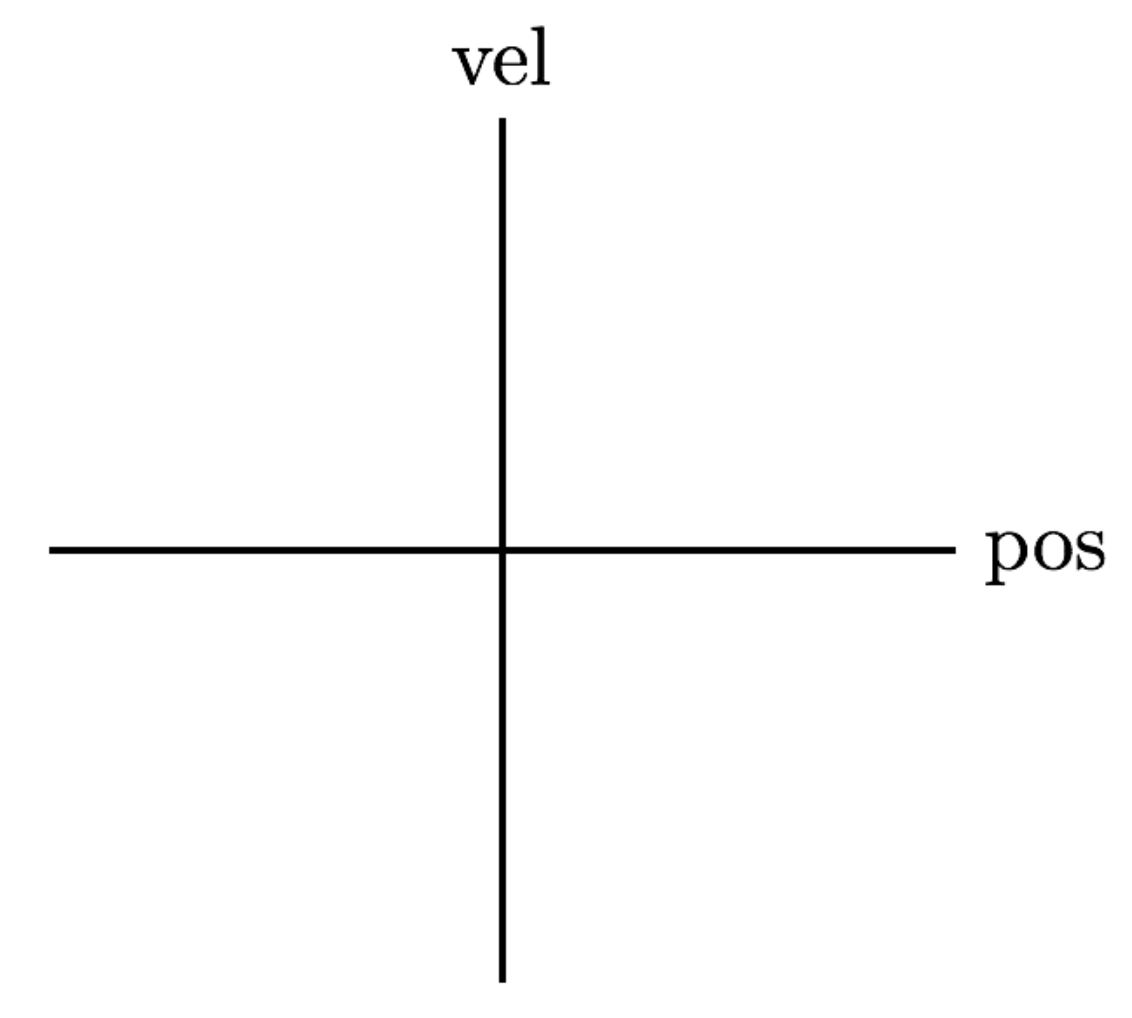
\includegraphics[width=1.75in]{10/10VelPos.png} \hspace{.25in} 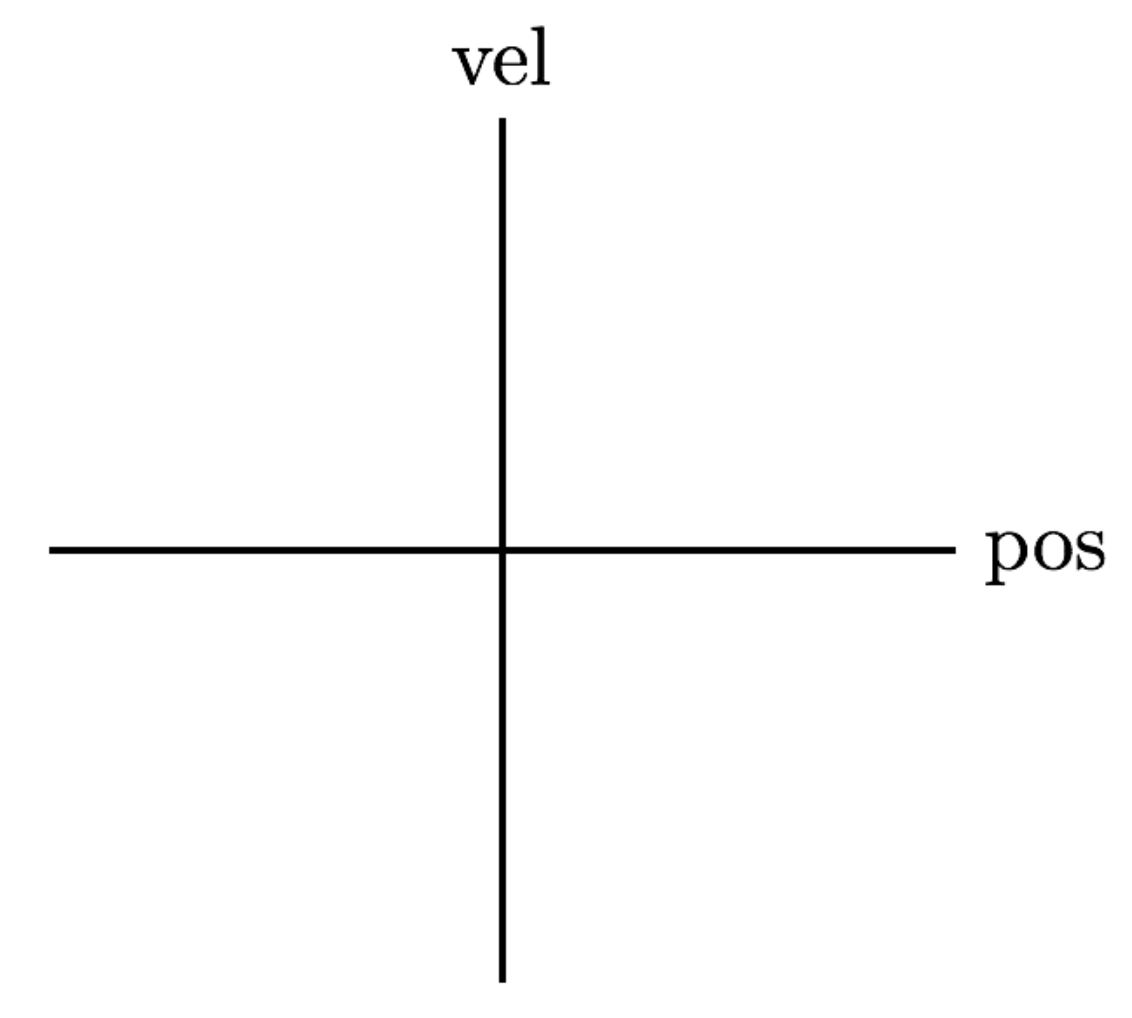
\includegraphics[width=1.75in]{10/10VelPos.png} 
\end{center}
\vfill

\item	Use Newton's Law of motion to develop a rate of change equation to model the motion of an object on a spring. Assume that the only forces acting on the object are the spring force ($-kx$, where $k$ is the spring constant) and the friction force (assumed to be proportional to the velocity, namely  $-b\frac{dx}{dt}$, where $b$ is the damping coefficient). \label{10problem2}
\vfill
\clearpage

\item	Application of Newton's Law of Motion to the spring-mass situation in the previous problem results in the following: 
\[\frac{d^2x}{dt^2}+\frac{b}{m}\frac{dx}{dt}+\frac{k}{m}x=0,\]
where $x$ is the position of the object attached to the end of the spring, $m$ is the mass of the object, $b$ is the friction parameter (also called damping coefficient), and $k$ is the spring constant. Because $\frac{dx}{dt} = y$, where $y$ is the velocity, and $\frac{dy}{dt} = \frac{d^2x}{dt^2}$, we can converting this to a system of two differential equations as follows:  \label{10problem3}
\begin{align*}
\frac{dx}{dt}&=y\\
\frac{dy}{dt}&= -\frac{k}{m}x-\frac{b}{m}y
\end{align*}
Use the GeoGebra applet \href{https://ggbm.at/vT5tgWrg}{\underline{https://ggbm.at/vT5tgWrg}} to investigate the motion of the object as depicted in the phase plane when $m = 1$, the spring constant $k = 2$, and the friction parameter, $b$, varies between 0 and 4. In particular, how does the vector field (and corresponding behavior of the mass) change when the friction parameter increases from 0 to say 2, 2.3, 3, or 3.8? Use the space below to record your observations.

\vspace{-1in}\hspace{-0.6in}
\includegraphics[width=0.5in]{10/10SpringMassExplorationQR.png} \\

\begin{center}
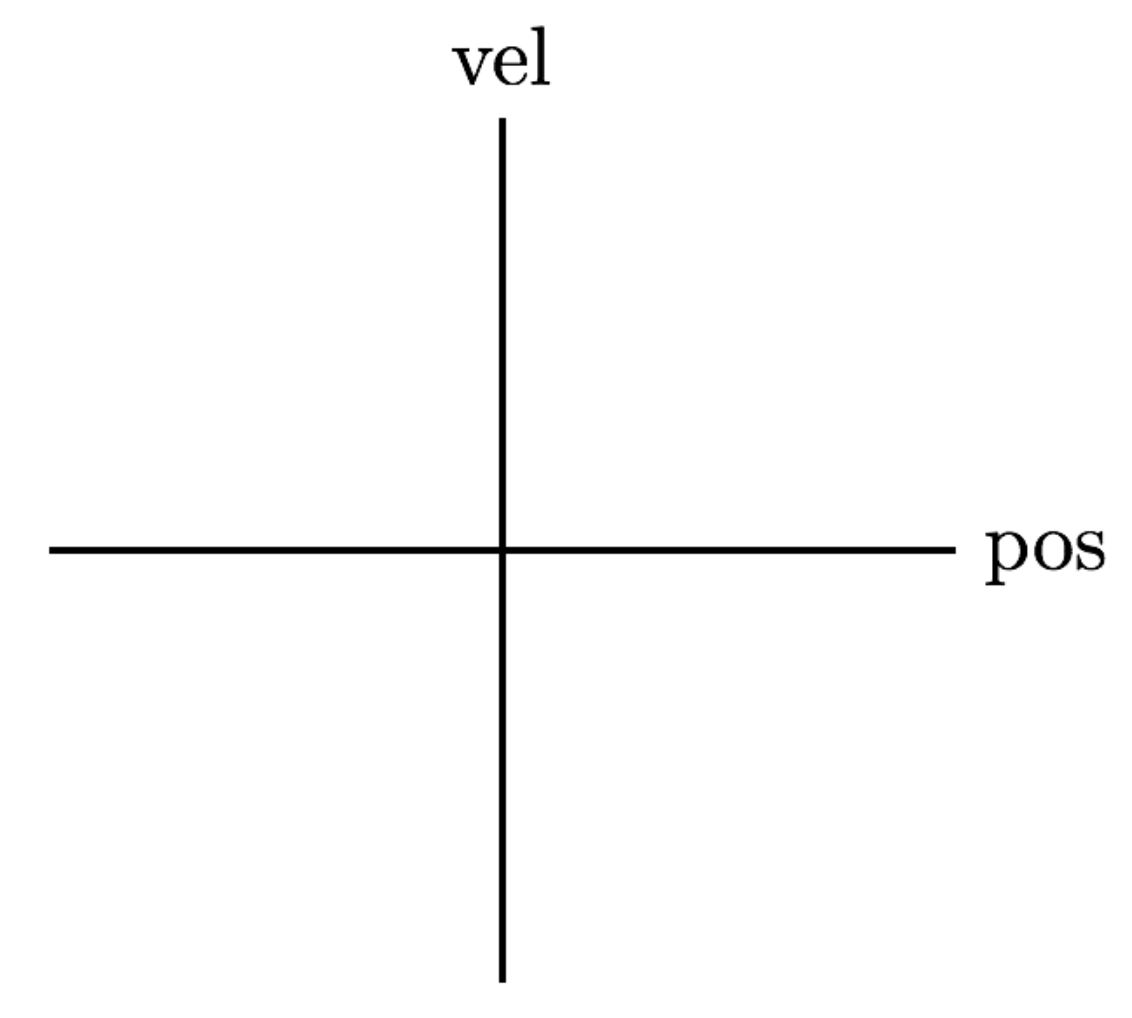
\includegraphics[width=2in]{10/10VelPos.png} \hspace{.25in} 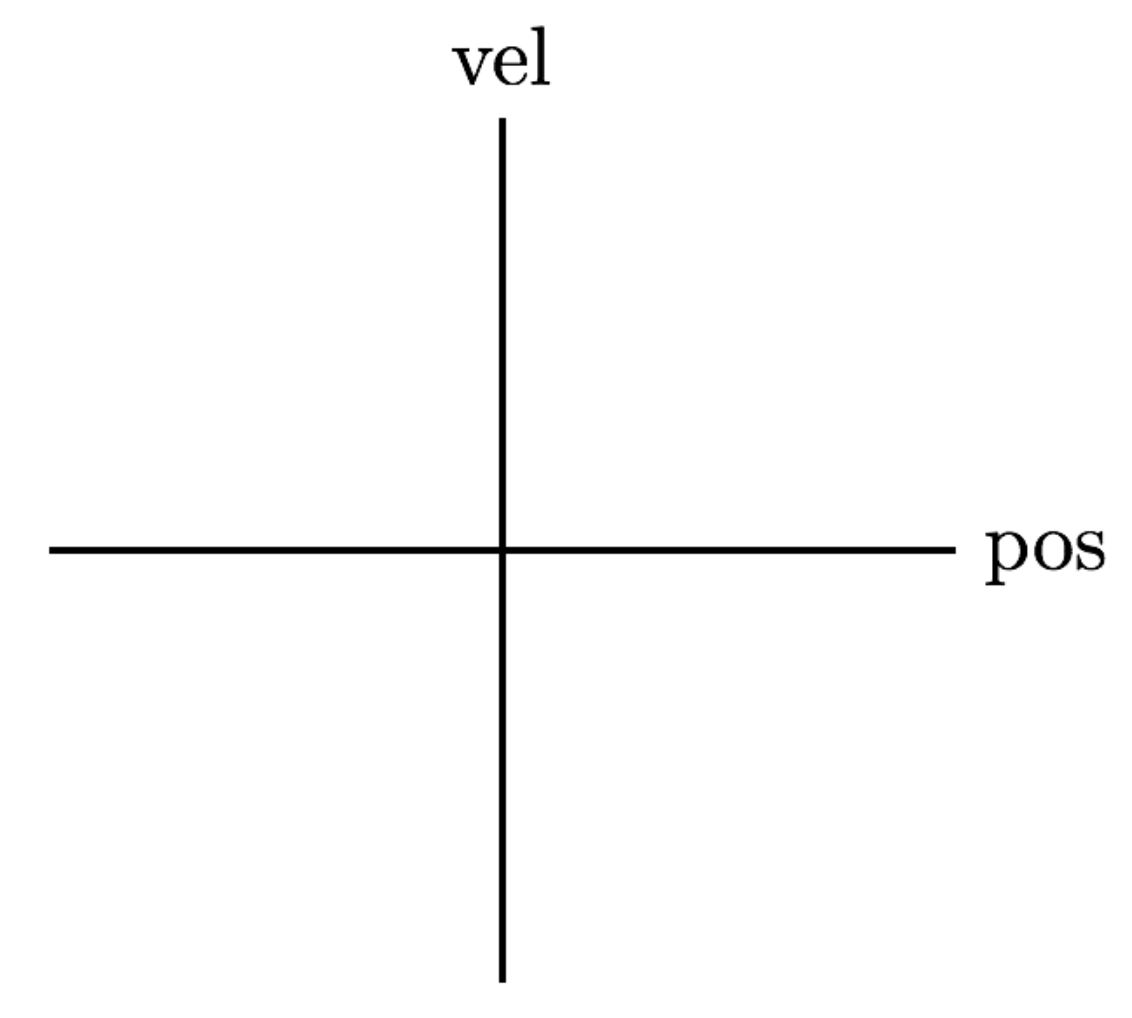
\includegraphics[width=2in]{10/10VelPos.png} \hspace{.25in} 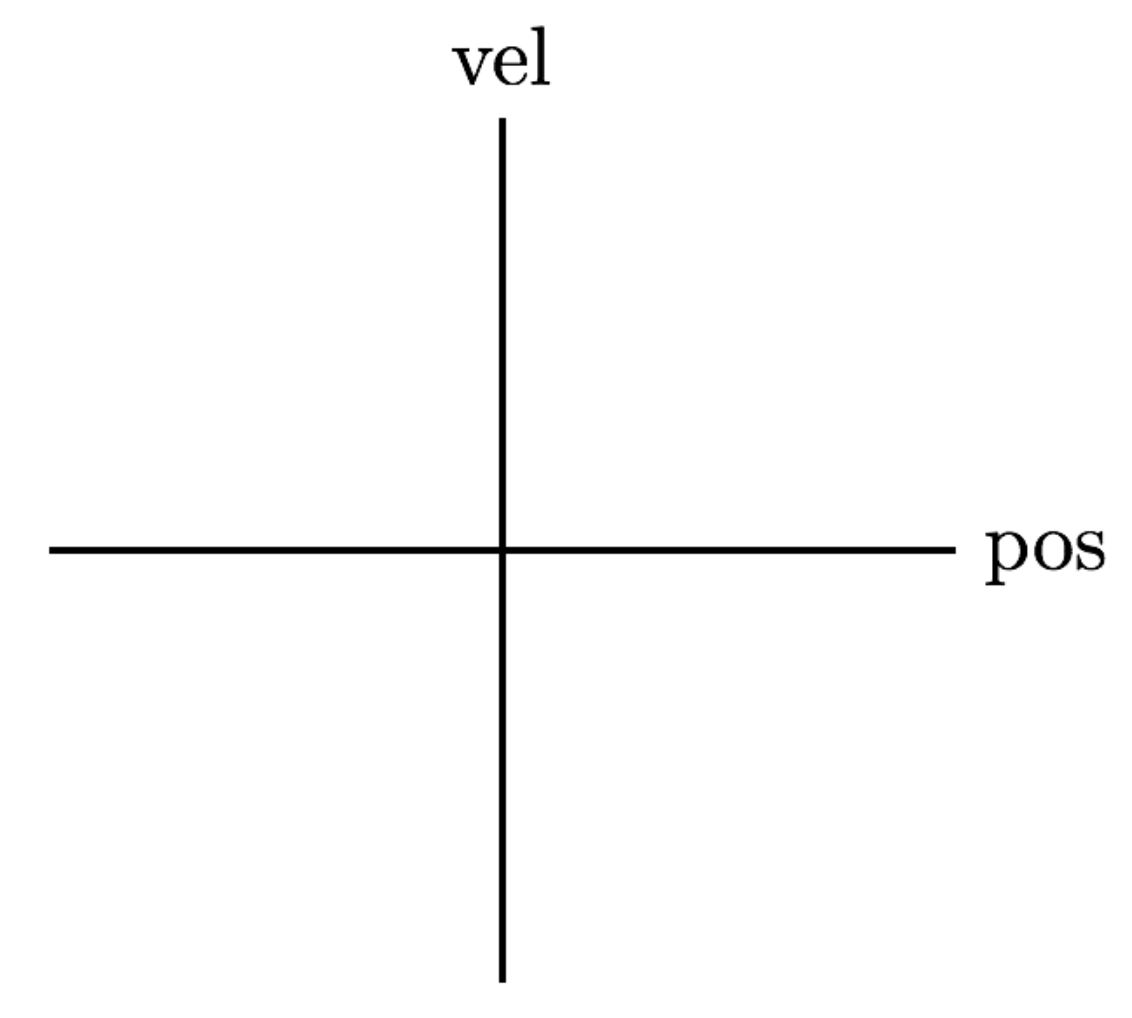
\includegraphics[width=2in]{10/10VelPos.png} 
\end{center}
\vfill
\clearpage

\item	Joey and Kara set the friction parameter to 3, resulting in the following system:
\begin{align*}
\frac{dx}{dt}&=y\\
\frac{dy}{dt}&= -2x-3y
\end{align*}
They notice that graphs of solutions in the position-velocity plane seem to get pulled into the origin along a straight line. Help Joey and Kara figure out how to use algebra to find the slope of this straight line.  \label{10problem4} \\

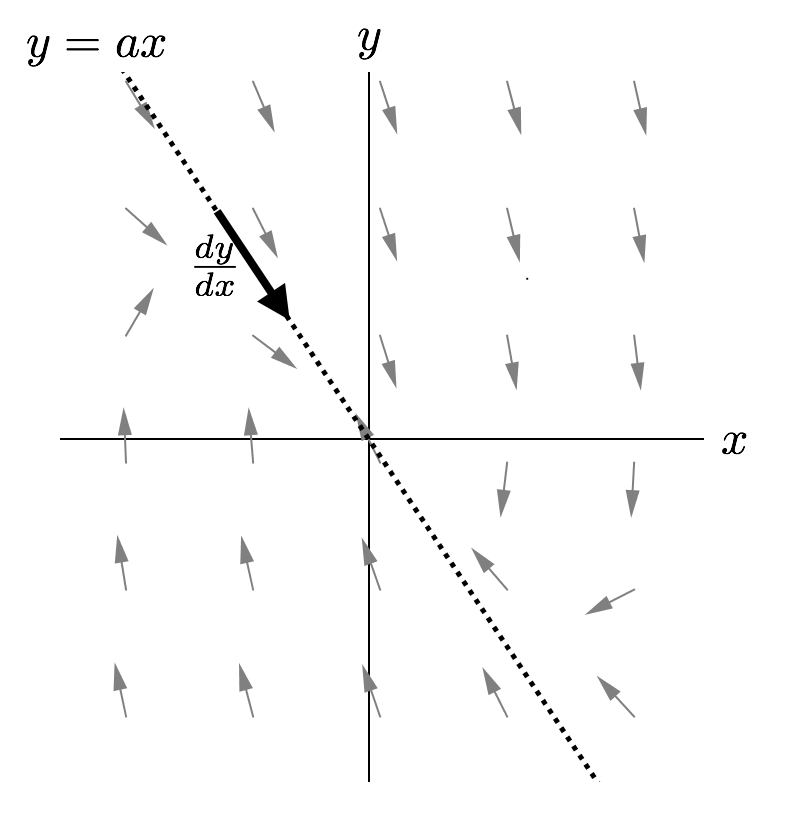
\includegraphics[width=4in]{10/10JoeyKara1.png}
\vfill

\clearpage
\item Continuing their investigation with the friction parameter set to 3, Kara and Joey are working to find the slope of the observed straight line. Joey sets up the equation $\displaystyle\frac{-2x-3y}{y}=\frac{y}{x}$ and Kara sets up the equation $\displaystyle\frac{-2x - 3ax}{ax} = a$. Interpret Joey's and Kara's equations and then solve both. \label{10problem5} \\

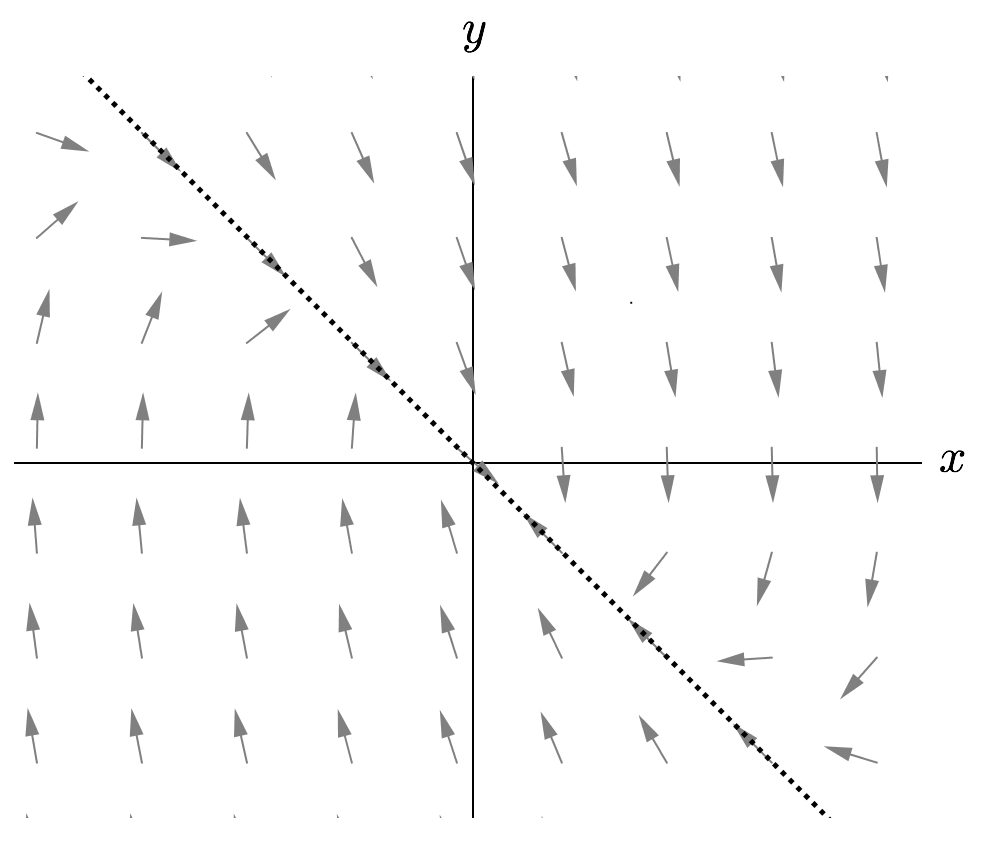
\includegraphics[width=4in]{10/10JoeyKara2.png}
\vfill
\item	Place your finger on the dotted line starting in the second quadrant and trace out the path that the mass takes, as represented in the phase plane. Describe what happens to your finger and relate this to the motion of the mass. \label{10problem6}
\vfill

\item	Joey found another straight line solution when the friction parameter $b$ was set to 1. Use algebra to find the slope or explain why he is mistaken. \label{10problem7}
\vfill
\clearpage

\item In your investigation of the spring-mass system 
\begin{align*}
\frac{dx}{dt}&=y\\
\frac{dy}{dt}&=-2x-3y
\end{align*}
you should have found that when the friction parameter was equal to 3, solutions with initial conditions that are either on the line $y = -x$ or on the line $y = -2x$ head directly toward the origin along a straight path. \label{10problem8}
\begin{center}
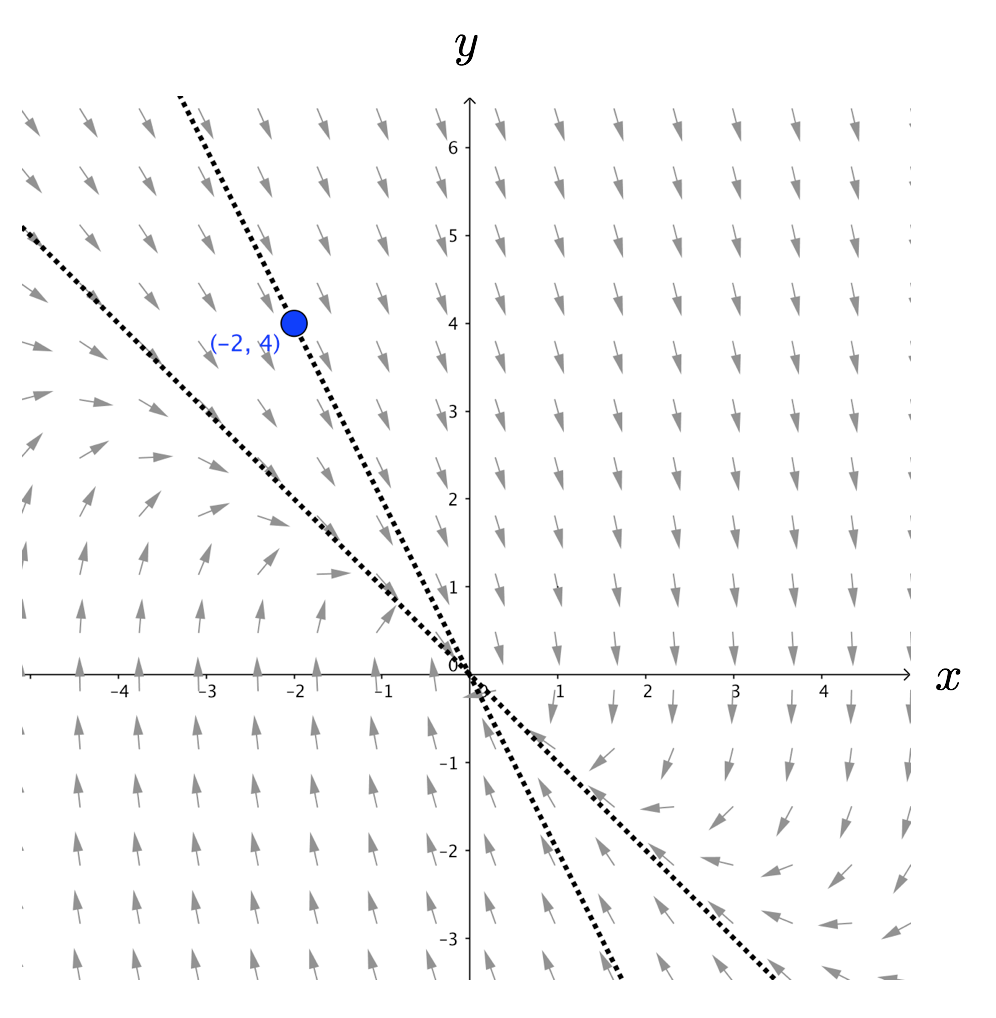
\includegraphics[width=4in]{10/10VectorField1.png}
\end{center}
For the initial condition (-2, 4), what are the equations for $ x(t)$ and $y(t)$? Hint: substitute $y=-2x$ and $x = -y/2$ into $dx/dt$ and $dy/dt$, respectively.
\vfill

\clearpage

\item	Susan notices that the $x(t)$ and $y(t)$ equations have the same exponent, and then makes the conjecture that along any straight line solution, $x(t)$ and $y(t)$ \textbf{must} have the same exponent. Do you agree with her conjecture? Why or why not?  \label{10problem9}
\vfill

\item \label{10problem10}
\begin{enumerate}
\item What are the $x(t)$ and $y(t)$ equations for the solution with initial condition (-1, 2)? What does the 3D graph of this solution look like?\label{10problem10parta}
\vfill
\item If you multiplied $x(t)$ and $y(t)$ equations from problem \ref{10problem10parta} by some number, say -3 for example, is the result also a solution to the system of differential equations? Algebraically show that your conclusion is correct. \label{10problem10partb}
\vfill
\item   What are the $x(t)$ and $y(t)$ equations for \textit{any} solution with initial condition along the line  $y = -2x$? \label{10problem10partc}
\vfill
\end{enumerate}
\item	For the initial condition (-2, 2), what are the equations for $x(t)$ and $y(t)$? What are the $x(t)$ and $y(t)$ equations for \textit{any} solution with initial condition along the line  $y = -x$? \label{10problem11}
��\vfill
\clearpage

\item \label{10problem12}
\begin{enumerate}
\item Suppose you were to start with an initial condition somewhere in the second quadrant between the two straight line solutions, say at (-4, 6). Sketch what you think the solution as viewed in the phase plane looks like and explain your reasoning. \label{10problem12parta}
\begin{center}
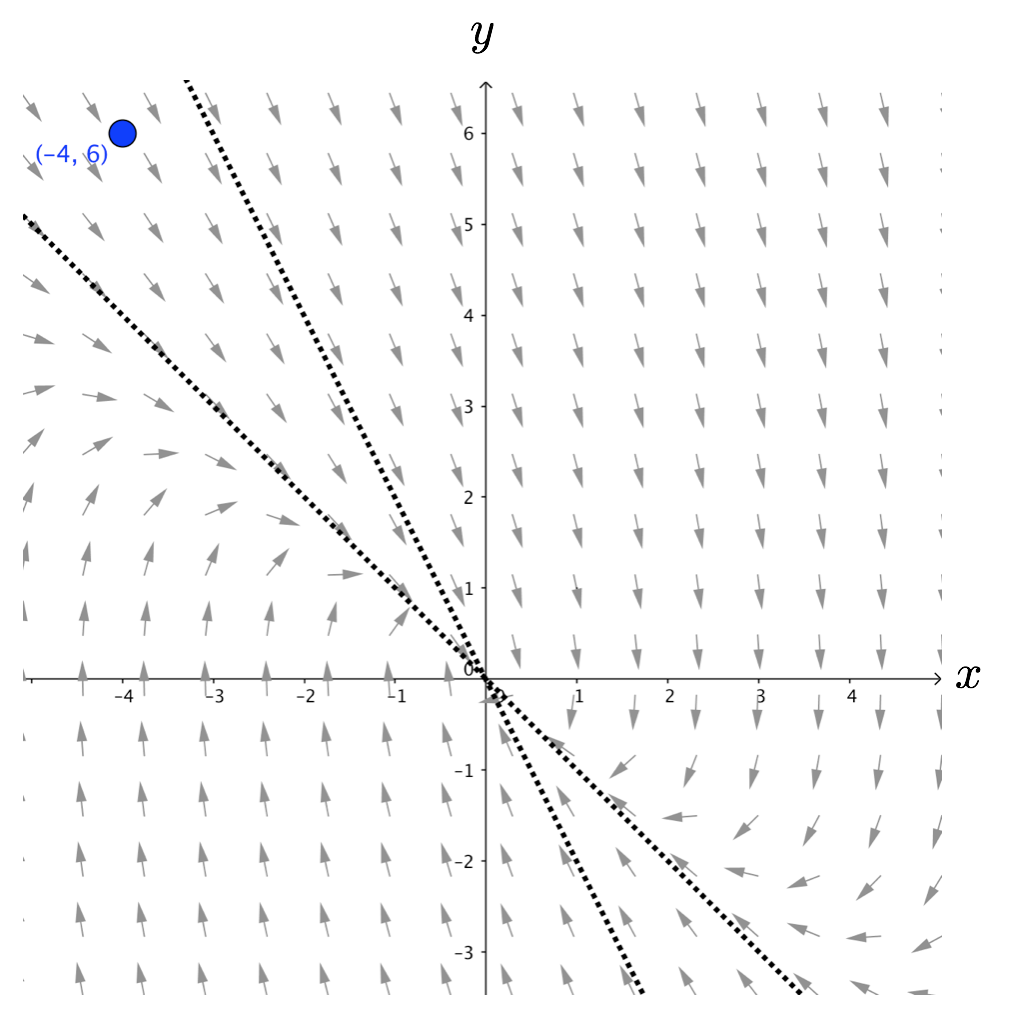
\includegraphics[width=4in]{10/10VectorField2.png}
\end{center}
\item Notice that $(-4,6)$ is a linear combination of the initial conditions $(-2,4)$ and $(-2,2)$, that is, $(-4,6)=(-2,4)+(-2,2)$. Show that the solution with the initial condition (-4, 6) is also a linear combination of the solutions with initial conditions $(-2,4)$ and $(-2,2)$. \label{10problem12partb}
\vfill
\item  According to your result in \ref{10problem12partb}, what does the solution in the phase plane look? Explain your reasoning. \label{10problem12partc}
\vfill
\end{enumerate}
\clearpage

\item \label{10problem13} \begin{enumerate}
\item What are the $x(t)$ and $y(t)$ equations for the solution with initial condition $(2,5)$? \label{10problem13parta}
\vfill
\item \textbf{According to your $x(t)$ and $y(t)$ equations}, what does the solution in the phase plane look like? Explain your reasoning and provide a sketch. Use the GeoGebra applet,\\ \href{https://ggbm.at/cMSUC7qR}{\underline{https://ggbm.at/cMSUC7qR}} to corroborate your conclusion. \label{10problem13partb}

\vspace{-.5in}\hspace{-.9in}
\includegraphics[width=0.5in]{10/10LinearCombinationsQR.png}
\vfill
\item Develop an argument that almost all graphs of solutions in the phase plane head into the origin with a slope of -1. \label{10problem13partc}
\vfill
\end{enumerate}
\clearpage
\item As a review of this unit, answer the following questions for the following system \label{10problem14}
\begin{align*}
\frac{dx}{dt} &= -3x+2y \\
\frac{dy}{dt} &= 6x+y
\end{align*}
\begin{enumerate}
\item Find the slopes of the straight line solutions.
\item For each straight line, find a solution.
\item Form the general solution.
\item In the phase plane sketch the straight line solutions and several non-straight line solutions.
\item How would you classify the equilibrium point?
\end{enumerate}
\end{enumerate}
\vfill

\clearpage

%%%%%%%%%%%%%%%%%%%%%%%%%%%%%%%%%%%%%%%%%
\pagebegin{Homework Set 10}

\begin{enumerate}
\item Consider the system from questions \ref{10problem3}-\ref{10problem7} from Unit 10. What is the smallest value of $b$ for which we get solutions that, when viewed in the position-velocity plane, lie along a straight line? Algebraically support your conclusion. \label{10HWproblem1}

\item Straight line Solutions for Systems of the Form 
\begin{align*}
\frac{dx}{dt}&=ax+by\\
\frac{dy}{dt}&=cx+dy
\end{align*}
Systems of equations of the form above are a special type of \textbf{linear system}. Linear systems model important applications, such as the spring mass system. Moreover, it is possible to find the general solution for any such linear system. For each of the system of differential equations below, address the following questions: \label{10HWproblem2}
\begin{itemize}

\item	How many equilibrium solutions are there are and what are they?

\item	Are there solutions that, when viewed in the phase plane (i.e., the $ x-y$ plane), lie along a straight line? If so, algebraically figure out the exact slope of the straight line(s). 

\item	For those systems that do have solutions that, when viewed in the phase plane, lie along a straight line, figure out the exact $x(t)$ and $y(t)$ equations for any solution with initial condition on the straight line(s). 

\item	For those systems that have straight line solutions, write down the general solution.

\item	How would you classify the equilibrium solution? Create terms if needed to classify any new types of equilibrium solutions and explain the meaning of your terms.

\item	For those systems of differential equations that do have solutions that, when viewed in the phase plane, lie along straight lines, what do these straight lines look like in 3D? Provide your best 3D sketch.

\end{itemize}

\begin{enumerate*}
\item $\displaystyle\begin{aligned} \frac{dx}{dt}&=-3x+2y\\
		\frac{dy}{dt}&=6x+y \end{aligned}$ \hspace{.15in}
\item $\displaystyle\begin{aligned} \frac{dx}{dt}&=x+y\\
		\frac{dy}{dt}&=-x+y \end{aligned}$ \hspace{.15in}
\item $\displaystyle\begin{aligned} \frac{dx}{dt}&=-2x-2y\\
		\frac{dy}{dt}&=-x-3y \end{aligned}$ \hspace{.15in}
\item $\displaystyle\begin{aligned} \frac{dx}{dt}&=2x+2y\\
		\frac{dy}{dt}&=x+3y \end{aligned}$
\end{enumerate*}

\clearpage

\item You figured out from our analysis on the previous problems, sometimes there are solutions in the phase plane that lie along a straight line headed directly towards or away from the equilibrium solution at the origin and sometimes there are not. \label{10HWproblem3}

\begin{enumerate}
\item	Explain in words how you figure out whether there are any straight line solutions in the phase plane and if so, what the slopes of this line or lines are. Demonstrate how your approach works in general for linear systems of the form \label{10HWproblem3parta}
\begin{align*}
\frac{dx}{dt}&=ax+by\\
\frac{dy}{dt}&=cx+dy
\end{align*}

\item	Explain in words how you figure out the $x(t)$ and $y(t)$ equations for any and all straight line solutions in the phase plane. Demonstrate how your approach works in general for linear systems of the form \label{10HWproblem3partb} 
\begin{align*}
\frac{dx}{dt}&=ax+by\\
\frac{dy}{dt}&=cx+dy
\end{align*}

\item	Explain in words why having two different straight line solutions is useful for finding the $x(t)$ and $y(t)$ equations for any initial condition. \label{10HWproblem3partc}
\end{enumerate}

\clearpage

\item	Below is a vector field for the system of differential equations:
\begin{align*}
\frac{dx}{dt}&=2x+3y\\
\frac{dy}{dt}&=-4y
\end{align*}
Straight line solutions lie along the line $y = 0$ (with positive exponent in the $x(t)$ and $y(t)$ equations) and along the line $y = -2x$ (with negative exponent in the $x(t)$ and $y(t)$ equations).
\begin{center}
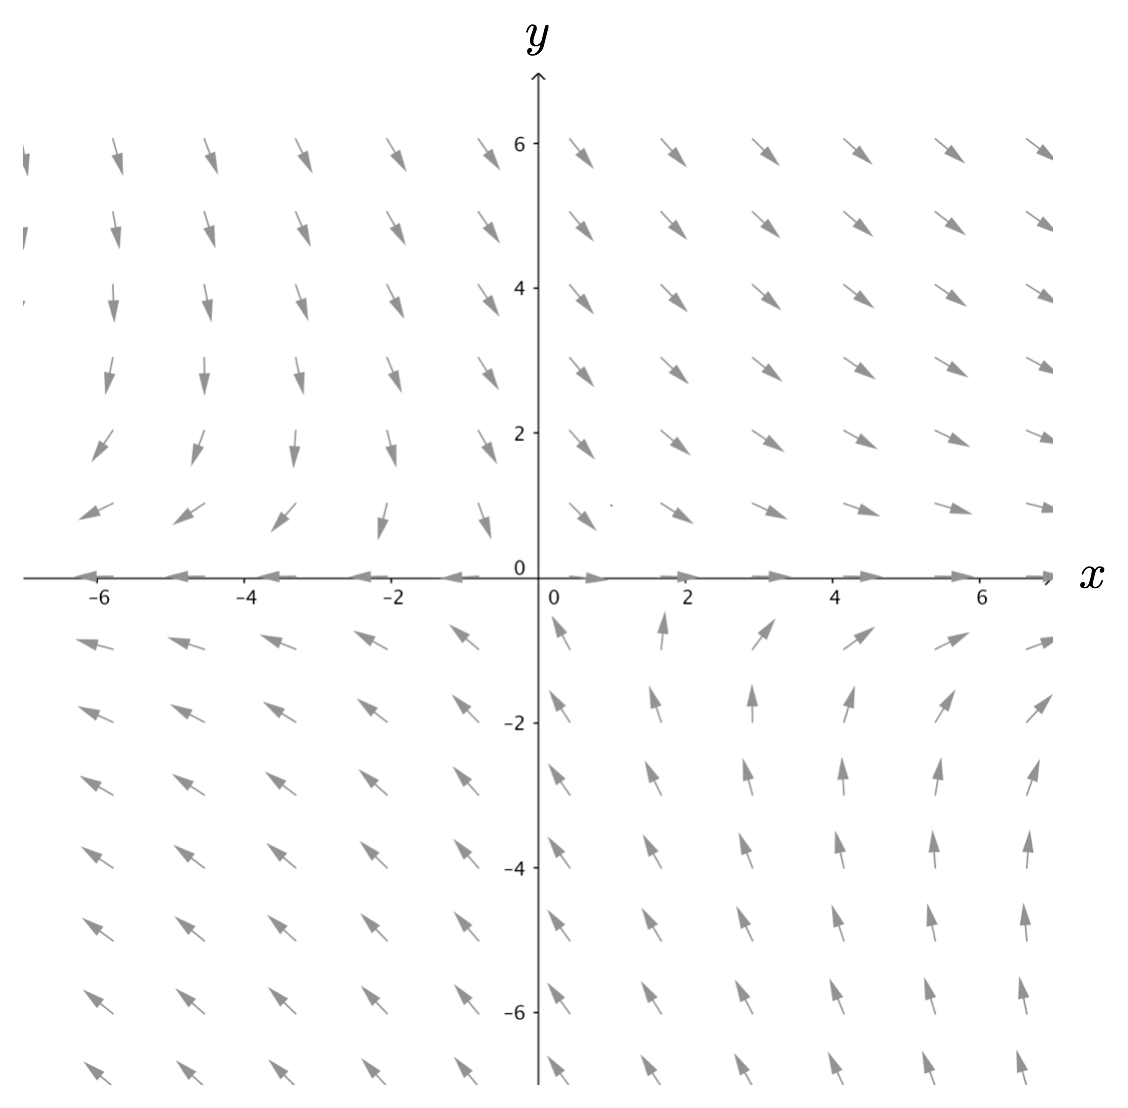
\includegraphics[width=4in]{10/10HWVectorField.png}
\end{center}
\begin{enumerate}
\item	Consider two different initial conditions, one at the point (1, 0) and one at the point (3, 0). Determine, with reasons, what happens to the graphs of the two solutions with these initial conditions as time progresses.\label{10HWproblem4parta} 
\item	Repeat problem \ref{10HWproblem4parta} for the initial conditions (-1, 2) and (-3, 6).\label{10HWproblem4partb}
��\vfill

\end{enumerate}

\clearpage

\item	Find a value or a range of values for the parameter $n$ between -4 and 4 (including non-integer values) in the system of differential equations \label{10HWproblem5}
\begin{align*}
\frac{dx}{dt}&= -3x+ny\\ \frac{dy}{dt}&= 6x+y
\end{align*}  
so that when you view solutions in the $x$-$y$ plane there are
\begin{enumerate}
\item exactly two different straight line solutions \label{10HWproblem5parta}
\item	no straight line solutions \label{10HWproblem5partb}
\item	exactly one straight line solution \label{10HWproblem5partc}
\item	an infinite number of equilibrium solutions and an infinite number of straight line solutions \label{10HWproblem5partd}
\end{enumerate}

\item	Consider the following system of differential equations: \label{10HWproblem6}
\begin{align*}
\frac{dx}{dt}&= 2x \\ \frac{dy}{dt}&= 2y
\end{align*}  
\begin{enumerate}
\item Without using technology, sketch many different solutions in the phase plane. Explain your reasoning.  \label{10HWproblem6parta}
\item	Unlike other systems of differential equations that we have been studying, this system can be solved using techniques from our study of 1-dimensional systems.  What makes this system different?  \label{10HWproblem6partb}
\item	Find the general solution in two ways, one using separation of variables and the other using straight line techniques. \label{10HWproblem6partc}
\item	Explain how the general solution can help you make sense of the solution graphs in the phase plane.  \label{10HWproblem6partd}
\end{enumerate}

\item Without using technology, sketch many different solutions in the phase plane for the following system of differential equations. Explain your reasoning. [\textit{Hint}: how many equilibrium solutions are there?] \label{10HWproblem7}

\begin{align*}
\frac{dx}{dt}&= -3x-\frac{1}{2}y \\ \frac{dy}{dt}&= 6x+y
\end{align*}

\clearpage

\item \textbf{A Swaying Skyscraper}: The following system of rate of change equations is a model for helping us make predictions about the motion of a tall building.
\begin{align*}
\frac{dx}{dt}&= y \\
\frac{dy}{dt}&= -x-y+x^3
\end{align*}
In this simplified system of rate of change equations, $x$ stands for the amount of displacement of the building from the vertical position at any time $t$ and $y$ stands for the horizontal velocity of the building at any time $t$. Use the GeoGebra Vector Field applet, \href{https://ggbm.at/kkNXUVds}{\underline{https://ggbm.at/kkNXUVds}}, as a tool to explore solutions as viewed in the $xy$-plane (i.e., the phase plane). \label{10HWproblem8}

\vspace{-.5in}\hspace{-.6in}
\includegraphics[width=0.5in]{10/10VectorFieldQR.png}

\begin{enumerate}
\item Determine all equilibrium solutions and explain the meaning of each one in terms of the swaying skyscraper. Create any terms needed to classify new types of equilibrium solutions and briefly explain your reasons or imagery behind your choice of terms. \label{10HWproblem8parta}
 
\item Provide a sketch of several representative curves in the phase plane and give an interpretation for the motion of the building for the different types of curves (e.g., does the building remain standing? If so, for what initial conditions? For what range of initial conditions is a disaster predicted?) \label{10HWproblem8partb}
\end{enumerate}

\end{enumerate}


